\chapter{Evaluación Experimental}
\label{capitulo4}
\lhead{Capítulo 4. \emph{Evaluación Experimental}}

Este capítulo consiste en la descripción de la metodología usada durante la evaluación de los métodos introducidos en los capítulos anteriores, así como el análisis de los resultados obtenidos de dicha evaluación. El objetivo de este estudio radica en la comparación empírica de cinco metaheurísticas (\emph{i.e.} GGA, SGA, CHC, PBIL y PSO) adaptadas para encontrar soluciones al problema de selección de instancias. Adicionalmente, se pretende estudiar el impacto de la aplicación de estrategias alternativas de generación de soluciones iniciales: disminuyendo la probabilidad de aparición de cada bit (de $50\%$ a $5\%$) y modificando dichas probabilidades en función de los subconjuntos de instancias generados por diferentes algoritmos heurísticos (\emph{i.e.} CNN, NEHS, ClosestNE y FarthestNE).

\section{Diseño Experimental}

La metodología seguida durante la evaluación experimental permite establecer la efectividad de las metaheurísticas descritas en función de
\begin{inparaenum}[\itshape a\upshape)]
\item la reducción del conjunto de instancias usado para el entrenamiento del clasificador (en este caso un clasificador 1-NN), y
\item la precisión de dicho clasificador --una vez entrenado-- al clasificar instancias previamente desconocidas.
\end{inparaenum}
La metodología experimental debe permitir la generalización del comportamiento de las diferentes metaheurísticas, así como las estrategias de generación de soluciones iniciales, con la finalidad de comparar los resultados obtenidos y establecer los métodos más efectivos frente al problema de selección de instancias.

\subsection{Conjuntos de datos}

Un factor esencial en la evaluación de métodos de selección de instancias es el conjunto de datos utilizado; la distribución de los datos, el número de instancias y atributos, y la cantidad de datos ruidosos, son solo algunos de los elementos que modifican el espacio de búsqueda del problema y por ende la efectividad de los algoritmos heurísticos para encontrar buenas soluciones. Los conjuntos de datos usados en este trabajo pertenecen al \emph{UCI Machine Learning Repository} \cite{BacheLichman:2013} y al \emph{KEEL Data-Mining Software Tool} \cite{alcala2010keel}.

Los 14 conjuntos seleccionados fueron separados en 3 grupos en función del número de instancias de cada conjunto. En la tabla \ref{data-small} se presentan 9 conjuntos con menor cantidad de instancias.

\begin{table}[h!]
\centering
\begin{tabular}{l c c c}
\hline
\textsc{Conjunto} & \textsc{Instancias} & \textsc{Atributos} & \textsc{Clases} \\
\hline
\hline
Cleveland & 297 & 13 &  5 \\
Glass     & 214 &  9 &  7 \\
Iris      & 150 &  4 &  3 \\
LED7Digit & 500 &  7 & 10 \\
Monk      & 432 &  6 &  2 \\
Pima      & 768 &  8 &  2 \\
WDBC      & 569 & 30 &  2 \\
Wine      & 178 & 13 &  3 \\
Wisconsin & 683 &  9 &  2 \\
\hline
\end{tabular}
\caption{Conjuntos de datos pequeños}
\label{data-small}
\end{table}

En la tabla \ref{data-med} se describen dos conjuntos de datos caracterizados como de tamaño medio.

\begin{table}[h!]
\centering
\begin{tabular}{l c c c}
\hline
\textsc{Conjunto} & \textsc{Instancias} & \textsc{Atributos} & \textsc{Clases} \\
\hline
\hline
Banana       &  5300 &  2 &  2 \\
Segmentation &  2100 & 19 &  7 \\
\hline
\end{tabular}
\caption{Conjuntos de datos medianos}
\label{data-med}
\end{table}

Finalmente, los 3 conjuntos con mayor número de instancias se presentan en la tabla \ref{data-big}.

\begin{table}[h!]
\centering
\begin{tabular}{l c c c}
\hline
\textsc{Conjunto} & \textsc{Instancias} & \textsc{Atributos} & \textsc{Clases} \\
\hline
\hline
Pen-Based    & 10992 & 16 & 10 \\
Satimage     &  6435 & 36 &  6 \\
Thyroid      &  7200 & 21 &  3 \\
\hline
\end{tabular}
\caption{Conjuntos de datos grandes}
\label{data-big}
\end{table}

\subsection{Particiones y ejecuciones}

Los conjuntos de datos considerados en la sección anterior son particionados usando la estrategia de validación cruzada en 10 iteraciones (10-\emph{fold cross-validation}). El conjunto inicial de instancias $T$ es dividido aleatoriamente en 10 conjuntos disjuntos de igual tamaño $T_1, T_2, \dots T_{10}$. Adicionalmente, cada conjunto $T_i$ se mantiene la proporción de distribución de las clases del conjunto original $T$. En función de esta partición, se definen un par de conjuntos $(T'_i, T_i)$, con $i = 1 \dots 10$, donde $T'_i = T \setminus T_i$.

El conjunto $T'_i$, también conocido como el conjunto de ``entrenamiento'', es usado por las metaheurísticas durante el proceso de búsqueda para evaluar soluciones intermedias; en vez de usar $T$, se usa el conjunto $T'_i$ como el conjunto de instancias inicial. Las instancias restantes, pertenecientes al conjunto $T_i$, son usadas como conjunto de ``validación'', \emph{i.e.} la mejor solución encontrada por las metaheurísticas es usada para clasificar las instancias --previamente desconocidas-- de $T_i$.

Cada metaheurística es evaluada usando los 10 pares de conjuntos $(T'_i, T_i)$. Por cada par de conjunto entrenamiento-validación se realizan 3 repeticiones. \emph{i.e.} un total de 30 ejecuciones de una metaheurística para un conjunto de datos y un tipo de inicialización particular.

\subsection{Parámetros}

\blindtext

\begin{table}[h!]
\centering
\begin{tabular}{l c c c c c}
\hline
\multirow{2}{*}{\textsc{Parámetros}}
	& \multicolumn{5}{c}{\textsc{Algoritmos}} \\\cline{2-6}
	& GGA & SGA & CHC & PBIL & PSO \\
\hline
\hline
Iteraciones        &  1000 &  1000 &  1000 &  1000 &  1000 \\
Población          &    50 &    30 &    30 &    40 &     5 \\
Prob. de Cruce     &   0.9 &   1.0 &     - &     - &     - \\
Prob. de Mutación  & 0.001 & 0.001 &     - & 0.001 &     - \\
Mutation Shift     &     - &     - &     - &  0.01 &     - \\
Learning Rate      &     - &     - &     - &   0.1 &     - \\
Neg. Learning Rate &     - &     - &     - &  0.01 &     - \\
Partículas         &     - &     - &     - &     - &     5 \\
Velocidad Máxima   &     - &     - &     - &     - &   0.2 \\
Inercia            &     - &     - &     - &     - &   0.9 \\
c1                 &     - &     - &     - &     - &   0.1 \\
c2                 &     - &     - &     - &     - &   0.1 \\
\hline
\end{tabular}
\caption{Parámetros usados en cada metaheurística}
\label{table-parameters}
\end{table}

\section{Resultados}

\blindtext

\subsection{Comparación entre inicializaciones}

\blindtext

\subsubsection{Probabilidad de aparición de bit (50\% \emph{vs} 5\%)}

\blindtext

\begin{table}[h!]
\centering
\begin{tabular}{c c c c c c}
\hline
\multirow{2}{*}{$\delta$}
	& \multirow{2}{*}{\textsc{Conjuntos}}
	& \textsc{Tiempo} & \textsc{Tamaño}
	& \multicolumn{2}{c}{$\%$ de \textsc{Error}} \\\cline{5-6}
 & & \scriptsize{(seg)} & \scriptsize{$100*\vert R \vert / \vert T \vert$}
	& \scriptsize{Entrenamiento} & \scriptsize{Validación} \\
\hline
\hline
\multirow{3}{*}{\ \ $50\%\ \ $}
 & Pen-based & 1515.50 & 38.17 & 0.38 &  0.91 \\
 & Satimage  & 1413.98 & 36.49 & 4.64 & 10.91 \\
 & Thyroid   & 1045.41 & 36.62 & 3.80 &  7.97 \\
\hline
\multicolumn{2}{l}{\emph{Promedio}} & 1324.96 & 37.09 & \textbf{2.94} & \textbf{6.60} \\
\hline
\multirow{3}{*}{$5\%$}
 & Pen-based & 1132.87 & 4.50 &  2.01 &  2.49 \\
 & Satimage  &  900.64 & 5.26 & 10.12 & 12.19 \\
 & Thyroid   &  646.20 & 4.26 &  6.62 &  7.16 \\
\hline
\multicolumn{2}{l}{\emph{Promedio}} & \textbf{893.24} & \textbf{4.67} & 6.25 & 7.28 \\
\hline
\end{tabular}
\caption{Parámetros usados en cada metaheurística}
\label{table-unif50vs5}
\end{table}

\blindtext

\begin{figure}[h!]
\centering
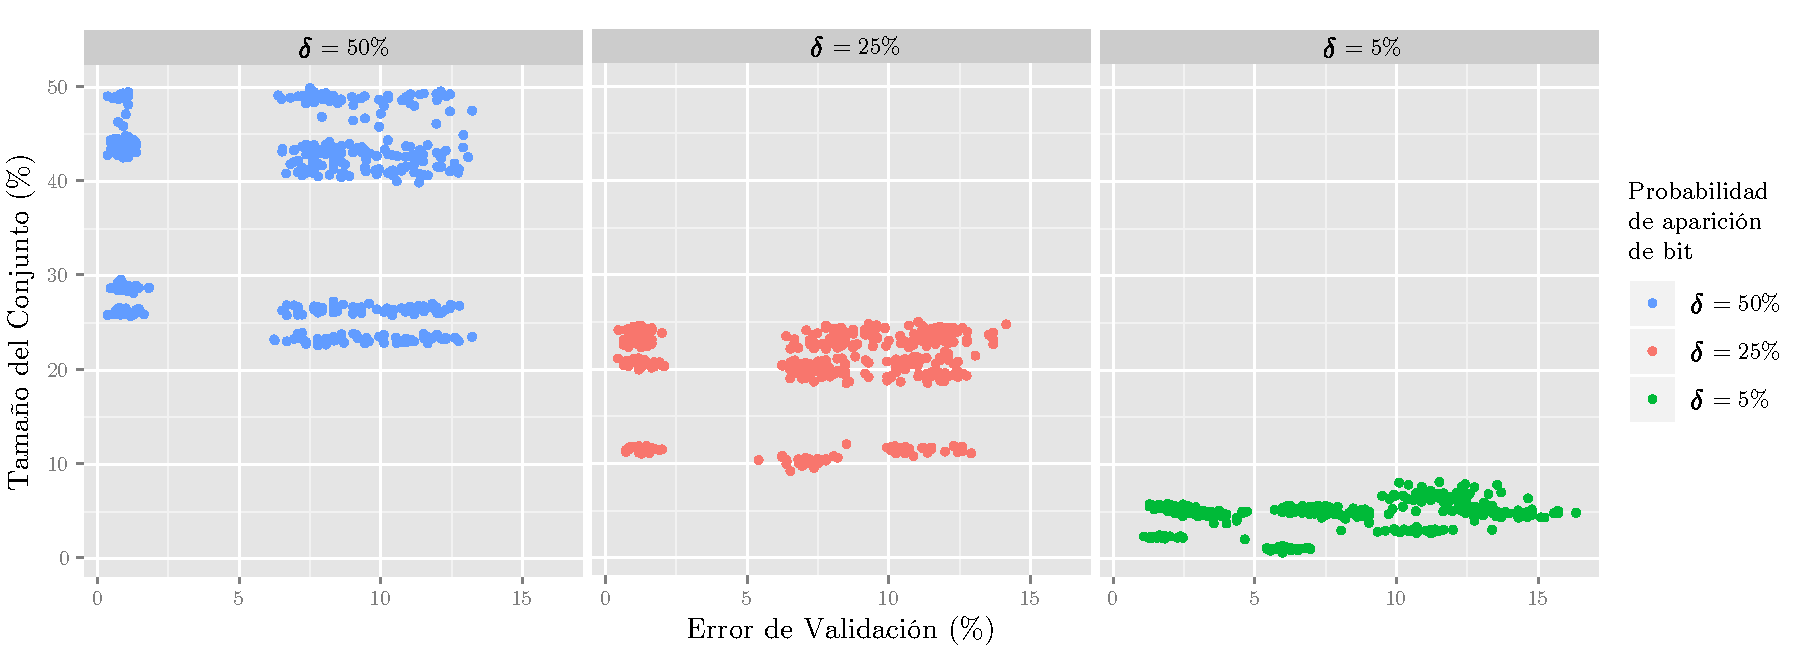
\includegraphics[width=0.7\textwidth]{uniforme.pdf}
\caption{Hola}
\label{fig-unif}
\end{figure}

\subsubsection{Inicialización usando algoritmos heurísticos}

\blindtext

\begin{table}[h!]
\centering
\begin{tabular}{l c c c c}
\hline
\multirow{2}{*}{\textsc{Inicialización}}
	& \textsc{Tiempo} & \textsc{Tamaño}
	& \multicolumn{2}{c}{$\%$ de \textsc{Error}} \\\cline{4-5}
 & \scriptsize{(seg)} & \scriptsize{$100*\vert R \vert / \vert T \vert$}
	& \scriptsize{Entrenamiento} & \scriptsize{Validación} \\
\hline
\hline
Uniforme   & \textbf{893.24} & \textbf{4.67} & 6.25 & \textbf{7.28} \\
NEHS       & 958.94 & 4.70 & \textbf{6.20} & \textbf{7.28} \\
CNN        & 921.68 & 5.11 & 6.27 & 7.85 \\
FarthestNE & 932.19 & 4.98 & 6.94 & 7.67 \\
ClosestNE  & 932.75 & 5.56 & 7.21 & 8.95 \\
\hline
\end{tabular}
\caption{Parámetros usados en cada metaheurística}
\label{table-inits}
\end{table}

\begin{figure}[h!]
\centering
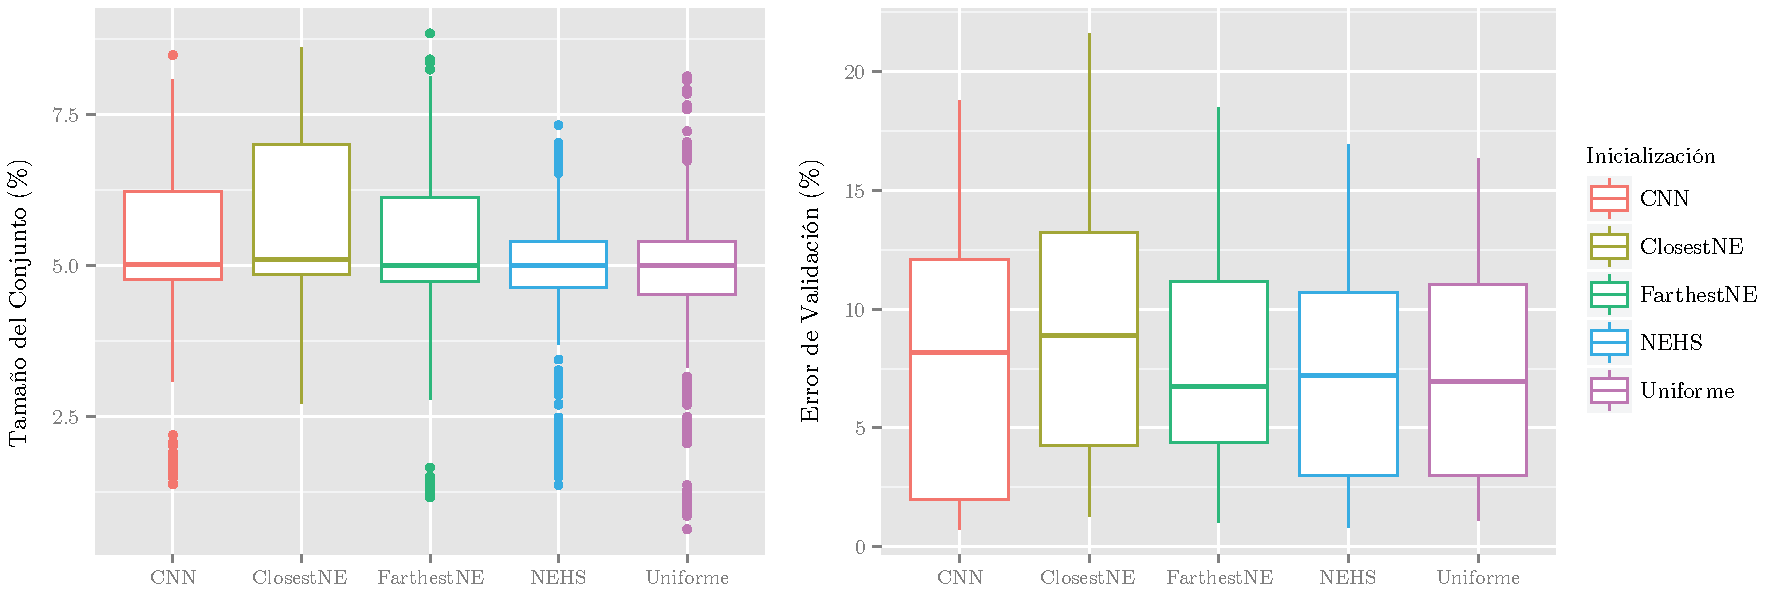
\includegraphics[width=\textwidth]{inits-boxplot.pdf}
\caption{Hola}
\label{fig-inits}
\end{figure}

\blindtext

\begin{table}[h!]
\centering
\begin{tabular}{l c c|l c c|l c c}
\hline
\multicolumn{3}{c|}{\textsc{Error de Validación}}
	& \multicolumn{3}{c|}{\textsc{Tamaño}}
	& \multicolumn{3}{c}{\textsc{Error + Tamaño}} \\
\hline
Inicialización & Rank & Mejor & Inicialización & Rank & Mejor & Inicialización & Rank & Mejor \\
\hline
\hline
NEHS       & 2.06 & 4 & Uniforme   & 1.86 & 6 & NEHS       & 2.00 & 5 \\
Uniforme   & 2.40 & 2 & NEHS       & 2.26 & 3 & Uniforme   & 2.20 & 2 \\
CNN        & 2.86 & 4 & FarthestNE & 2.86 & 4 & CNN        & 2.93 & 4 \\
FarthestNE & 2.93 & 5 & CNN        & 3.60 & 2 & FarthestNE & 3.06 & 4 \\
ClosestNE  & 4.73 & 0 & ClosestNE  & 4.40 & 0 & ClosestNE  & 4.80 & 0 \\
\hline
\end{tabular}
\caption{Parámetros usados en cada metaheurística}
\label{table-inits-rank}
\end{table}

\blindtext

\subsection{Comparación entre metaheurísticas}

\blindtext

\subsubsection{Conjuntos pequeños}

\blindtext

\begin{table}[h!]
\centering
\begin{tabular}{l c c c c}
\hline
\multirow{2}{*}{\textsc{Algoritmo}}
	& \textsc{Tiempo} & \textsc{Tamaño}
	& \multicolumn{2}{c}{$\%$ de \textsc{Error}} \\\cline{4-5}
 & \scriptsize{(seg)} & \scriptsize{$100*\vert R \vert / \vert T \vert$}
	& \scriptsize{Entrenamiento} & \scriptsize{Validación} \\
\hline
\hline
GGA  &  5.51 & 4.66 & \textbf{10.94} & \textbf{17.89} \\
SGA  & \textbf{0.70} & 4.85 & 13.23 & 18.94 \\
CHC  &  1.75 & 3.44 & 14.15 & 19.45 \\
PBIL &  2.95 & \textbf{3.36} & 13.32 & 18.64 \\
PSO  & 10.59 & 6.28 & 18.64 & 21.90 \\
\hline
\end{tabular}
\caption{Parámetros usados en cada metaheurística}
\label{res-small}
\end{table}

\blindtext

\begin{table}[h!]
\centering
\begin{tabular}{l c c|l c c|l c c}
\hline
\multicolumn{3}{c|}{\textsc{Error de Validación}}
	& \multicolumn{3}{c|}{\textsc{Tamaño}}
	& \multicolumn{3}{c}{\textsc{Error + Tamaño}} \\
\hline
Algoritmo & Rank & Mejor & Algoritmo & Rank & Mejor & Algoritmo & Rank & Mejor \\
\hline
\hline
PBIL & 2.00 & 4 & PBIL & 1.44 & 5 & PBIL & 1.55 & 6 \\
GGA  & 2.22 & 4 & CHC  & 1.88 & 3 & GGA  & 2.44 & 2 \\
SGA  & 2.66 & 1 & GGA  & 3.11 & 1 & CHC  & 2.88 & 0 \\
CHC  & 3.77 & 0 & SGA  & 3.88 & 0 & SGA  & 3.22 & 1 \\
PSO  & 4.33 & 0 & PSO  & 4.66 & 0 & PSO  & 4.88 & 0 \\
\hline
\end{tabular}
\caption{Parámetros usados en cada metaheurística}
\label{res-small-rank}
\end{table}

\blindtext

\subsubsection{Conjuntos medianos}

\blindtext

\begin{table}[h!]
\centering
\begin{tabular}{l c c c c}
\hline
\multirow{2}{*}{\textsc{Algoritmo}}
	& \textsc{Tiempo} & \textsc{Tamaño}
	& \multicolumn{2}{c}{$\%$ de \textsc{Error}} \\\cline{4-5}
 & \scriptsize{(seg)} & \scriptsize{$100*\vert R \vert / \vert T \vert$}
	& \scriptsize{Entrenamiento} & \scriptsize{Validación} \\
\hline
\hline
GGA  & 80.49 & 6.02 &  \textbf{5.96} &  8.58 \\
SGA  & \textbf{8.67} & 5.80 &  6.76 &  8.92 \\
CHC  &  8.89 & 4.46 &  7.51 &  8.90 \\
PBIL & 38.06 & \textbf{2.72} &  6.06 &  \textbf{8.35} \\
PSO  & 97.98 & 5.55 & 10.66 & 11.83 \\
\hline
\end{tabular}
\caption{Parámetros usados en cada metaheurística}
\label{res-med}
\end{table}

\blindtext

\begin{table}[h!]
\centering
\begin{tabular}{l c c|l c c|l c c}
\hline
\multicolumn{3}{c|}{\textsc{Error de Validación}}
	& \multicolumn{3}{c|}{\textsc{Tamaño}}
	& \multicolumn{3}{c}{\textsc{Error + Tamaño}} \\
\hline
Algoritmo & Rank & Mejor & Algoritmo & Rank & Mejor & Algoritmo & Rank & Mejor \\
\hline
\hline
PBIL & 1.5 & 1 & PBIL & 1.0 & 2 & PBIL & 1.0 & 2 \\
GGA  & 2.5 & 1 & CHC  & 2.0 & 0 & CHC  & 2.0 & 0 \\
SGA  & 3.0 & 0 & PSO  & 3.0 & 0 & GGA  & 3.5 & 0 \\
CHC  & 3.0 & 0 & GGA  & 4.5 & 0 & SGA  & 3.5 & 0 \\
PSO  & 5.0 & 0 & SGA  & 4.5 & 0 & PSO  & 5.0 & 0 \\
\hline
\end{tabular}
\caption{Parámetros usados en cada metaheurística}
\label{res-med-rank}
\end{table}

\blindtext

\subsubsection{Conjuntos grandes}

\blindtext

\begin{table}[h!]
\centering
\begin{tabular}{l c c c c}
\hline
\multirow{2}{*}{\textsc{Algoritmo}}
	& \textsc{Tiempo} & \textsc{Tamaño}
	& \multicolumn{2}{c}{$\%$ de \textsc{Error}} \\\cline{4-5}
 & \scriptsize{(seg)} & \scriptsize{$100*\vert R \vert / \vert T \vert$}
	& \scriptsize{Entrenamiento} & \scriptsize{Validación} \\
\hline
\hline
GGA  & 1938.78 & 5.58 & 6.11 & 7.13 \\
SGA  &  152.71 & 5.74 & 5.42 & 6.56 \\
CHC  & \textbf{22.37} & 5.00 & 7.35 & 8.08 \\
PBIL &  472.63 & \textbf{2.36} & \textbf{4.35} & \textbf{6.19} \\
PSO  & 2208.22 & 4.80 & 7.76 & 8.43 \\
\hline
\end{tabular}
\caption{Parámetros usados en cada metaheurística}
\label{res-big}
\end{table}

\blindtext

\begin{table}[h!]
\centering
\begin{tabular}{l c c|l c c|l c c}
\hline
\multicolumn{3}{c|}{\textsc{Error de Validación}}
	& \multicolumn{3}{c|}{\textsc{Tamaño}}
	& \multicolumn{3}{c}{\textsc{Error + Tamaño}} \\
\hline
Algoritmo & Rank & Mejor & Algoritmo & Rank & Mejor & Algoritmo & Rank & Mejor \\
\hline
\hline
PBIL & 1.00 & 3 & PBIL & 1.00 & 3 & PBIL & 1.00 & 3 \\
SGA  & 2.00 & 0 & PSO  & 2.00 & 0 & SGA  & 2.00 & 0 \\
GGA  & 3.00 & 0 & CHC  & 3.00 & 0 & GGA  & 3.33 & 0 \\
CHC  & 4.33 & 0 & GGA  & 4.33 & 0 & CHC  & 4.33 & 0 \\
PSO  & 4.66 & 0 & SGA  & 4.66 & 0 & PSO  & 4.33 & 0 \\
\hline
\end{tabular}
\caption{Parámetros usados en cada metaheurística}
\label{res-big-rank}
\end{table}

\blindtext

\subsubsection{Análisis de los resultados}

\blindtext

\begin{table}[h!]
\centering
\begin{tabular}{l c c c c c c c c c c}
\hline
\multirow{2}{*}{\textsc{Conjunto}}
	& \multicolumn{2}{c}{GGA}
	& \multicolumn{2}{c}{SGA}
	& \multicolumn{2}{c}{CHC}
	& \multicolumn{2}{c}{PBIL}
	& \multicolumn{2}{c}{PSO}\\\cline{2-11}
 & \scriptsize{Error} & \scriptsize{Tam.}
 & \scriptsize{Error} & \scriptsize{Tam.}
 & \scriptsize{Error} & \scriptsize{Tam.}
 & \scriptsize{Error} & \scriptsize{Tam.}
 & \scriptsize{Error} & \scriptsize{Tam.}\\
\hline
\hline
%            GGA             SGA            CHC            PBIL           PSO             
Banana       & 10.83 &  5.33 & 10.60 & 5.33 & 10.67 & 4.68 & \textbf{10.37} & \textbf{1.95} & 11.80 &  4.87 \\
Cleveland    & 45.81 &  6.02 & 43.92 & 5.18 & 44.81 & 3.70 & \textbf{43.16} & \textbf{3.21} & 44.53 &  5.63 \\
Glass        & \textbf{32.49} & 10.19 & 32.85 & 9.38 & 36.55 & \textbf{6.31} & 35.02 & 6.99 & 35.38 & 13.43 \\
Iris         &  5.11 &  {2.66} &  \textbf{4.44} & 3.00 &  5.11 & 2.93 &  6.22 & 2.78 &  4.66 &  4.86 \\
Led7digit    & 26.03 &  4.84 & 26.89 & 4.88 & 26.10 & \textbf{3.10} & \textbf{25.37} & 3.15 & 30.25 &  6.71 \\
Monk         & \textbf{11.16} &  6.57 & 18.67 & 7.26 & 19.16 & \textbf{4.53} & 17.88 & 4.85 & 29.40 &  7.49 \\
Pen-based    &  2.46 &  5.10 &  1.84 & 5.52 &  2.99 & 4.93 & \textbf{1.59} & \textbf{2.32} &  3.03 &  4.86 \\
Pima         & 27.43 &  5.08 & 27.91 & 5.48 & 26.35 & 4.04 & \textbf{26.26} & \textbf{3.68} & 30.08 &  4.97 \\
Satimage     & 11.80 &  6.49 & 11.21 & 6.40 & 12.92 & 5.18 & \textbf{10.58} & \textbf{3.04} & 14.00 &  4.77 \\
Segmentation & \textbf{6.33} &  6.72 &  7.25 & 6.26 &  7.12 & 4.23 &  6.34 & \textbf{3.48} & 11.85 &  6.24 \\
Thyroid      &  7.15 &  5.16 &  6.63 & 5.29 &  8.34 & 4.90 & \textbf{6.40} & \textbf{1.71} &  8.26 &  4.76 \\
WDBC         & \textbf{6.91} &  2.97 &  8.43 & 3.82 &  8.43 & 2.64 &  7.32 & \textbf{2.27} & 13.23 &  4.84 \\
Wine         & \textbf{3.17} &  2.82 &  4.53 & 3.03 &  5.08 & 2.95 &  3.93 & \textbf{2.62} &  6.00 &  4.76 \\
Wisconsin    &  2.88 &  0.81 &  2.83 & 1.66 &  3.46 & 0.75 & \textbf{2.63} & \textbf{0.68} &  3.60 &  3.86 \\
\hline
\emph{Promedio} & 14.25 & 5.05 & 14.86 & 5.18 & 15.51 & 3.92 & 14.50 & 3.05 & 17.58 & 5.86\\
\hline
\end{tabular}
\caption{Parámetros usados en cada metaheurística}
\label{res-big}
\end{table}

\begin{figure}[h!]
\centering
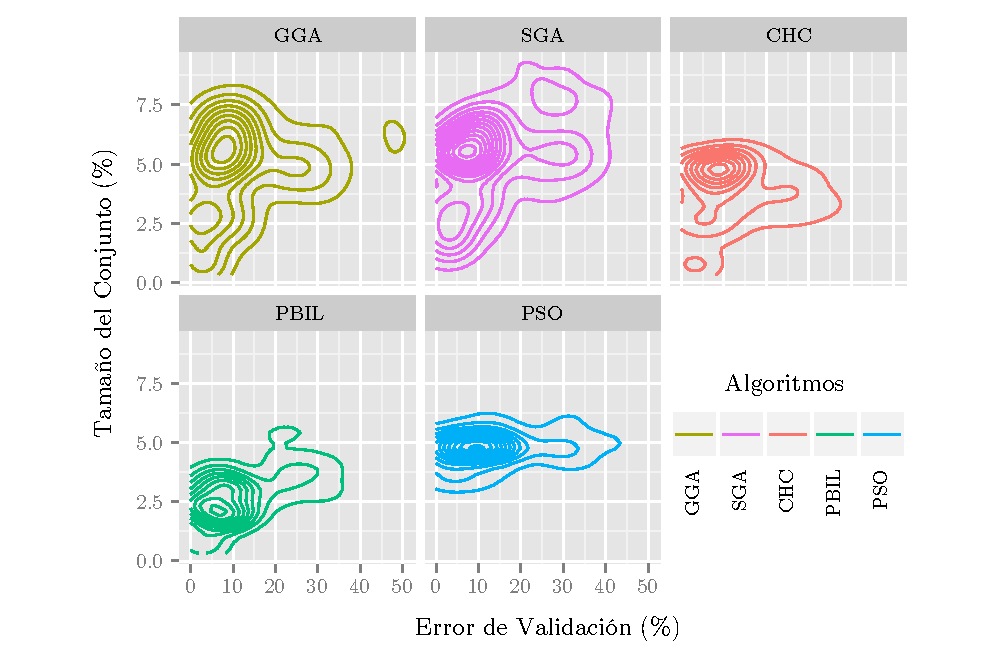
\includegraphics[width=\textwidth]{alg-density.pdf}
\caption{Hola}
\label{fig-alg-density}
\end{figure}
